\documentclass{amu_these}

\begin{document}

%% page de titre
	\chead{}
	\pdfbookmark[0]{Page de titre}{titre}
	\titlepage
\usefont{T1}{cmbr}{m}{n}\selectfont{}
\vspace*{-2cm}
\begin{center}
	\begin{minipage}[c]{0.25\linewidth}
		\raggedright 
\includegraphics[height=50px]{logo_amu}
	\end{minipage}\hfill
	\begin{minipage}[c]{0.25\linewidth}
		\raggedleft 
\includegraphics[height=50px]{int}
	\end{minipage}\hfill 
\end{center}
\begin{flushleft}
        \vspace{0.2cm}
    \LARGE UNIVERSITE D’AIX-MARSEILLE\\
        \vspace{0.2cm}
    \Large ECOLE DOCTORALE\\
        \vspace{0.2cm}
    \normalsize FACULTE\\
        \vspace{0.2cm}
    LABORATOIRE/UNITE DE RECHERCHE\\
    \begin{center}
        \vspace{2cm}
    THESE DE DOCTORAT\\
    \end{center}
        \vspace{0.5cm}
    Discipline :\\
    Spécialité :\\
    \begin{center}
        \vspace{0.5cm}
    \Large Prénom NOM\\
        \vspace{1cm}
    \large Titre de la thèse : sous-titre\\
    \end{center}
        \vspace{3cm}
    \normalsize Soutenue le 01 janvier 2012\\
        \vspace{0.4cm}
    Composition du jury :\\
\end{flushleft}
\vspace{0.4cm}
\begin{tabular}{lll}
Prénom NOM & Affiliation & Président du Jury \\
    \vspace{0.08cm}
Prénom NOM & Affiliation & Rapporteur \\
    \vspace{0.08cm}
Prénom NOM & Affiliation & Rapporteur \\
    \vspace{0.08cm}
Prénom NOM & Affiliation & Examinateur \\
    \vspace{0.08cm}
Prénom NOM & Affiliation & Examinateur \\
    \vspace{0.08cm}
Prénom NOM & Affiliation & Directeur de thèse \\
\end{tabular}
\usefont{T1}{bch}{m}{n}\selectfont{}
%% licence
	\newpage
	\thispagestyle{empty}
	~\vfill
\begin{center}
	\begin{minipage}[c]{0.25\linewidth}
		\raggedright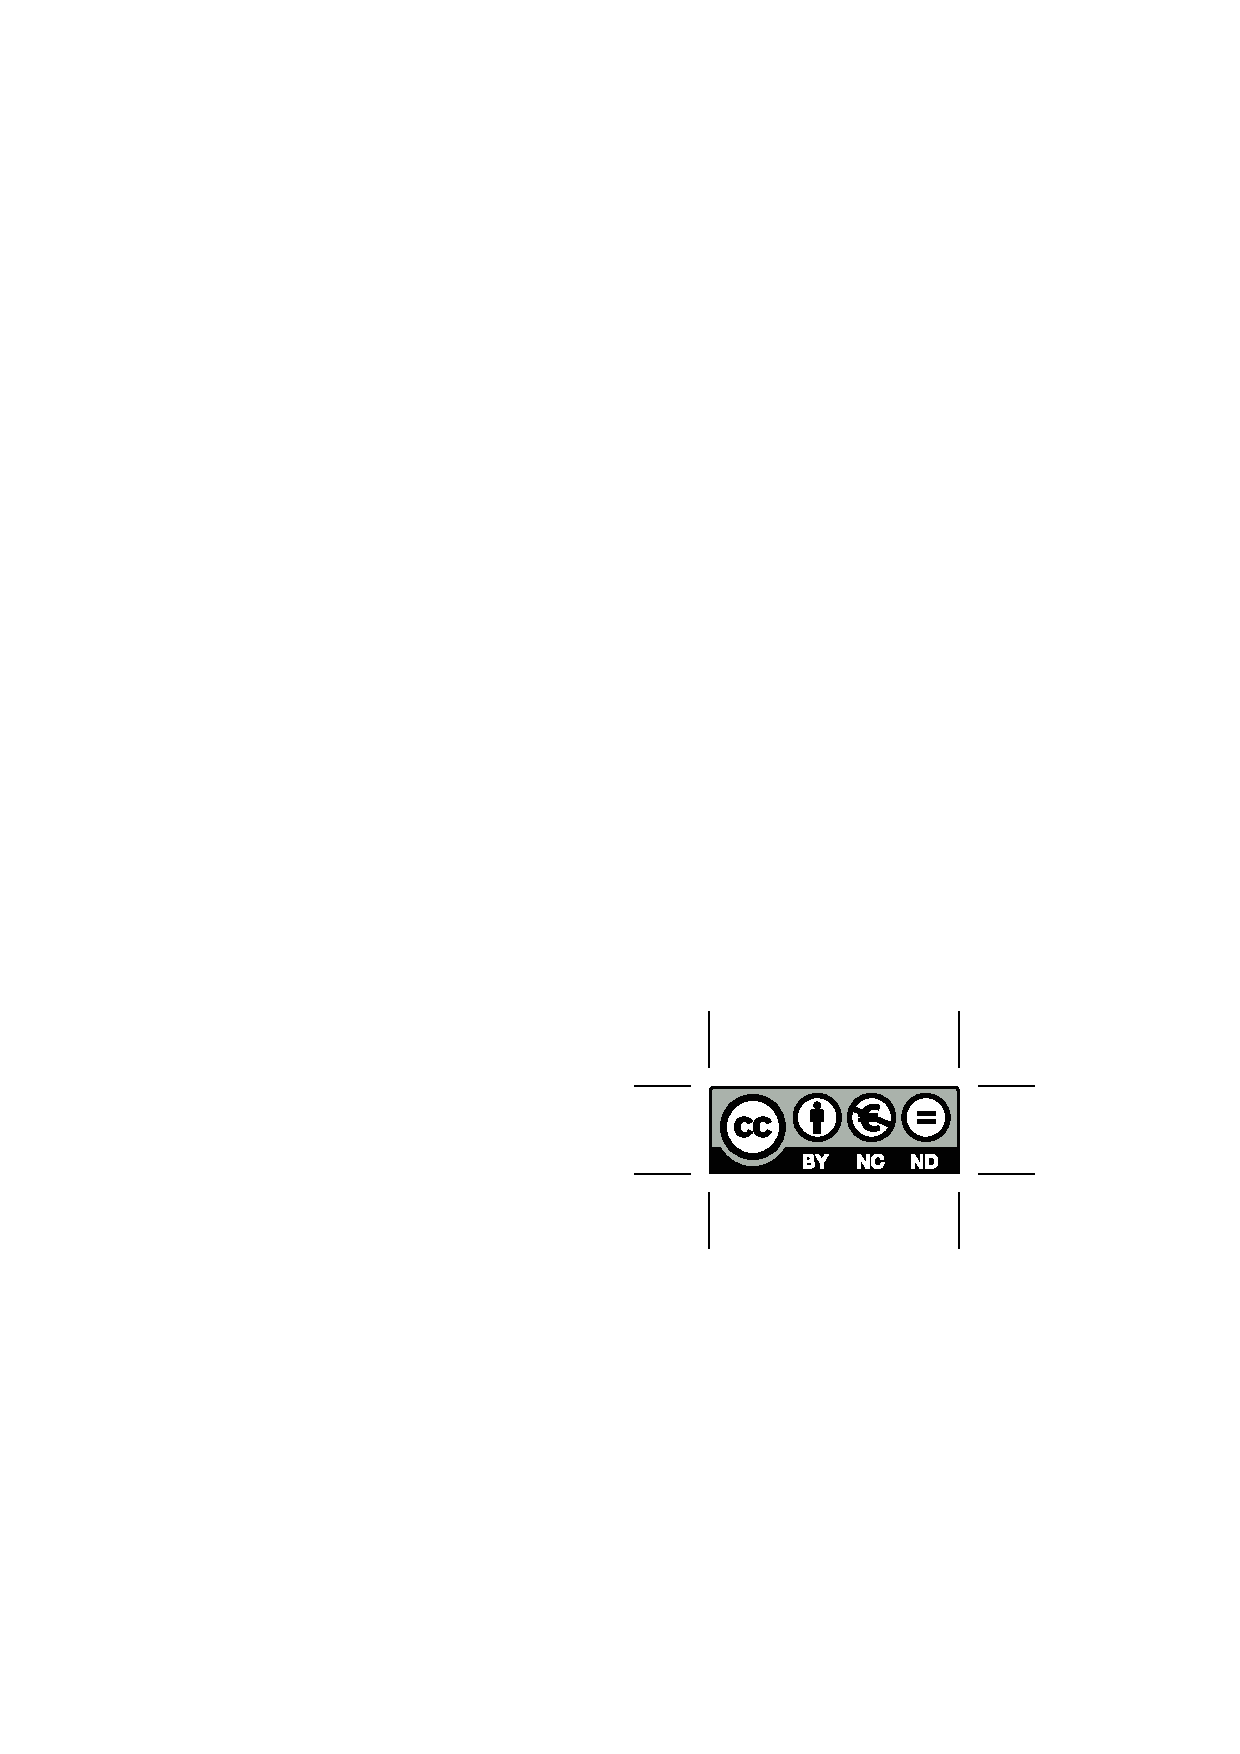
\includegraphics[height=35px]{by-nc-nd-eu}
	\end{minipage}\hfill
\end{center}

Cette oeuvre est mise à disposition selon les termes de la \href{https://creativecommons.org/licenses/by-nc-nd/4.0/deed.fr}{Licence Creative Commons Attribution - Pas d’Utilisation Commerciale - Pas de Modification 4.0 International}.

%% résumé
	\chapter*{Résumé}
	\lipsum[1]

\vspace{0.5cm}
Mots clés : géométrie algorithmique, complexe planaire et rectangulaire, géodésique, courbure globale non-positive
	\addcontentsline{toc}{chapter}{Résumé}
%% abstract
	\chapter*{Abstract}
	\selectlanguage{english}
\lipsum[1]\index{Lorem ipsum}

\vspace{0.5cm}
Keywords: computational geometry, planar and rectangular complex, geodesic, global nonpositive curvature
\selectlanguage{french}

	\addcontentsline{toc}{chapter}{Abstract}
%% remerciement
	\chapter*{Remerciements}
	Le modèle de thèse AMU n'existerait pas sans la contribution des doctorants. Nous souhaitons remercier tout particulièrement \href{http://www.theses.fr/2011AIX20720}{Mickaël Bojados}, \href{http://www.theses.fr/2011AIX22111}{Flora Cordoleani} et \href{http://www.theses.fr/2014AIXM4013}{Florian Caullery} pour leur aide précieuse et la qualité de leurs fichiers sources LaTeX.

\lipsum[1-2]\index{Nam dui ligula}

	\addcontentsline{toc}{chapter}{Remerciements}

%% désactive la protrusion localement (TOCLOFT NOMENCL)
    \microtypesetup{protrusion=false}
%% TOC
	\newpage
	\pdfbookmark[0]{Table des matières}{tdm}
	\tableofcontents
%% LOF
	\listoffigures
%% LOT
	\listoftables
%% Nomenclature
	%\nomenclature{$+a$}{Opérateur}
\nomenclature{$2a$}{Nombre}
\nomenclature{$:a$}{Symbole de ponctuation}
\nomenclature{$Aa$}{Lettre majuscule}
\nomenclature{$aa$}{Lettre minuscule}
\nomenclature{$\alpha$}{Lettre grecque}

\printnomenclature

		% Liste des acronymes, glossaire et liste des symboles (dans l'ordre)		
		\printglossary[type=\acronymtype , title={Liste des acronymes}, toctitle={Liste des acronymes}]
		\printglossary[title=Glossaire,toctitle=Glossaire]
		\printglossary[type=notation,title={Nomenclature}, toctitle={Nomenclature}]
%% rétabli la protrusion
    \microtypesetup{protrusion=true}

%%%% corps
	\chapter*{Introduction}
	\lipsum[1-2]
	\addcontentsline{toc}{chapter}{Introduction}

	\chapter{ Généralités}
	\section{Généralités sur la fusion thermonucléaire}
Lors d'une réaction de fusion, deux noyaux légers s'assemblent pour former un noyau plus lourd. Pour obtenir une réaction de fusion, il faut rapprocher suffisamment deux noyaux qui, puisqu'ils sont tous deux chargés positivement, se repoussent. Une certaine énergie est donc indispensable pour franchir cette barrière et arriver dans la zone, très proche du noyau, où se manifeste l'interaction forte capable de l'emporter sur la répulsion électrostatique.
\\ %  retour à la ligne
La réaction de fusion la plus favorable est celle faisant intervenir le deutérium et le tritium: $$_{1}^{2}D^{+}~+~_{1}^{3}T^{+}~\rightarrow ~_{2}^{4}He^{2+}~(3,5\,\textrm{MeV})~+~n~(14,1\,\textrm{MeV}).$$
\noindent % pas d'indentation en début de paragraphe
\lipsum[1]\index{Lorem ipsum}
\section{Deuxième section de la première partie}
\lipsum[2]


	\chapter{ Méthodologie de la recherche}
	\section{Matériel et méthodes}
\subsection{Modèle animal}
\lipsum[1]
\subsection{Traitement expérimental}
\subsubsection{Hypergravité}
\label{hypergravite} % on peut mettre systématiquement un \label après chaque titre de partie au cas où un /ref{} serait nécessaire
L'hypergravité consiste à augmenter la force du vecteur gravitaire en lui sur-imposant la force centrifuge. En effet, la force centrifuge induite par la rotation se surimpose à la gravité terrestre ce qui permet d'avoir une force résultante dépendante de la vitesse de rotation. On utilise pour cela des centrifugeuses qui sont des carrousels équipés de nacelles suspendues à des axes libres permettant à la force résultante d'être perpendiculaire au plancher de la nacelle et ainsi obtenir une \og gravité \fg{} dont la force est supérieure à la gravité terrestre tout en maintenant, pour les individus expérimentaux, l'orientation \og naturelle \fg{} de celle-ci.
\lipsum[1-5]
Une première note de fin de document\endnote{Première note de fin de document.} et une seconde\endnote{Deuxième note de fin de document.} et ... \endnote{... note de fin de document.} \endnote{... note de fin de document.} \endnote{... note de fin de document.} \endnote{... note de fin de document.} \endnote{... note de fin de document.} \endnote{... note de fin de document.} \endnote{... note de fin de document.} \endnote{... note de fin de document.} \endnote{... note de fin de document.} Quisque ullamcorper placerat ipsum.\endnote{\lipsum[3]}.
\subsubsection{La centrifugeuse}
Les caractéristiques techniques de la \index{centrifugeuse} ont été décrites dans un article de \cite{jamon_ground-based_2008} et dans la partie \ref{hypergravite}. Brièvement, la centrifugeuse (Figure~\ref{photo_centrifugeuse}) est de grand diamètre (jusqu'à 3,6~m en rotation). Pour limiter les vibrations, la centrifugeuse repose sur des dispositifs anti-vibrations. Le bruit produit par la centrifugeuse est faible. A un mètre de distance, le niveau sonore n'est que de 58~dB contre 52~dB si la centrifugeuse est arrêtée. Les nacelles sont sur des axes libres et chacune peut contenir trois cages de type standard (364x206x131 mm) avec 4 souris par cage, soit un total de 48 souris. La centrifugeuse est équipée de caméras infra-rouge couplées à un système de vidéo-surveillance accessible sur internet. Cela nous permet de contrôler les niveaux d'eau et de nourriture ainsi que de conduire des études de l'activité des individus expérimentaux à distance, de jour comme de nuit. La quantité d'eau et de nourriture disponible par cage permet de faire fonctionner la centrifugeuse 3 semaines sans interruption. Les animaux ont à disposition 400~g de nourriture et 500~ml d'eau, mais la consommation de nourriture sur cette période est en moyenne de 209~g ($\pm$14), et la consommation d'eau de 258 ml ($\pm$21) pour une cage de 4 souris. 
\begin{figure}[h!tbp] % à voir
\vspace{0.5cm}
\setcapindent{2em}
  \centering
  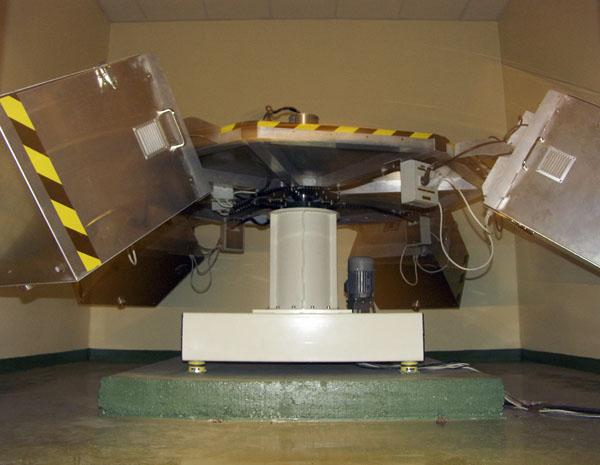
\includegraphics[width=0.7\textwidth]{photo_centrifugeuse}
  \caption[Photographie de la centrifugeuse]{Photographie de la centrifugeuse utilisée.}
  \label{photo_centrifugeuse}
\end{figure}
\lipsum[1]
\section{Deuxième section de la deuxième partie}
\lipsum[2]
\subsection{Première sous-section de la deuxième section de la deuxième partie}
\lipsum[4]
\subsection[Sous-sous-sous-partie 2]{Deuxième sous-section de la deuxième section de la deuxième partie} % entre [] pour affichage dans la TOC
\lipsum[4]Une note de bas de page\footnote{première note de bas de page} et une seconde\footnote{deuxième note de bas de page}.
\subsubsection{Ce titre de section ne s'affiche pas dans la TOC : tocdepth=2}
Nam dui ligula, fringilla a, euismod sodales, sollicitudin vel, wisi \parencite{zohdy_mapping_2012}. \lipsum[3] % citation entre parenthèses et tous les auteurs
\paragraph{Ce titre de section n'est pas numéroté : secnumdepth=3}~~\\ % "~~\\" fait le saut de ligne après le titre de 'paragraph'

% ce saut de ligne dans le code indente 'paragraph'
\lipsum[3]


	\chapter{ Résultats}
	Voir (Tableaux~\ref{table:alpha}~et~\ref{table:multi}).
\lipsum[3]
\begin{table}[h!tbp]
\begin{center}
\begin{tabular}{|c | c | c |}
\hline
$\lambda$ (nm) & $(\alpha_{\lambda}/\alpha_{426,7})_{moy}$ & écart type \\
\hline
391,9 \& 392,1 & 0,12 & 0,01 \\
588,9 \& 589,2 & 0,45 & 0,07 \\
657,8 \& 658,3 & 6,70 & 0,06 \\
711,3 & 0,16 & 0,01 \\
711,6 & 0,15 & 0,01 \\
712 & 0,31 & 0,02 \\
\hline
\end{tabular}
\end{center}
\caption[Valeur moyenne et écart type des rapports $\alpha_{\lambda}/\alpha_{426,7}$]{Valeur moyenne et écart type des rapports $\alpha_{\lambda}/\alpha_{426,7}$ mesurés pour les chocs plasma de la deuxième série.}
\label{table:alpha}
\end{table}

\lipsum[2]

Ajout d'une nouvelle entrée d'index de la centrifugeuse\index{centrifugeuse}.


	\chapter*{Conclusion}
	\chapter*{Conclusion}
\addcontentsline{toc}{chapter}{Conclusion}
\lipsum[1-2]
	\addcontentsline{toc}{chapter}{Conclusion}
%%%%

	\appendix
%% bibliographie
	\newpage
	\nocite{godard_borreliose_2012,leveque_winsor_2012} % ajoute à la biblio des ref non cités
\printbibliography
%% index
	\newpage
	\printindex
%% notes
	\newpage
	\printendnotes
%% annexes
	\setcounter{chapter}{0}
	\renewcommand{\thesection}{\Alph{section}}
	\chapter*{ANNEXES}
	\newpage
	\addcontentsline{toc}{chapter}{ANNEXES}
	\section{Intitulés des doctorats AMU}

		\begin{itemize}
		\item Discipline
			\begin{itemize}
			\item Spécialité
			\end{itemize}
		\end{itemize}
		
	\subsection*{ED 62 SCIENCES DE LA VIE ET DE LA SANTE}\label{ed-62-sciences-de-la-vie-et-de-la-sante}

		\begin{itemize}
		\item Biologie santé
			\begin{itemize}
			\item Biochimie structurale
			\item Génomique et  Bioinformatique
			\item Biologie du développement
			\item Immunologie
			\item Génétique
			\item Microbiologie
			\item Biologie végétale
			\item Neurosciences
			\item Oncologie
			\item Maladies infectieuses
			\item Pathologie vasculaire et nutrition
			\item Ethique
			\item Recherche clinique et Santé Publique
			\item Biotechnologie
			\end{itemize}
		\end{itemize}

	\subsection*{ED 67 SCIENCES JURIDIQUES ET POLITIQUES}\label{ed-67-sciences-juridiques-et-politiques}

		\begin{itemize}
		\item Droit
			\begin{itemize}
			\item Droit Privé
			\item Droit Public
			\item Histoire du Droit
			\end{itemize}
		\item Science Politique
		\end{itemize}

	\subsection*{ED 184 MATHEMATIQUES ET INFORMATIQUE}\label{ed-184-mathematiques-et-informatique}

		\begin{itemize}
		\item Mathématiques
		\item Informatique
		\item Automatique
		\end{itemize}

	\subsection*{ED 250 SCIENCES CHIMIQUES DE MARSEILLE}\label{ed-250-sciences-chimiques-de-marseille}

		\begin{itemize}
		\item Sciences Chimiques
		\end{itemize}

	\subsection*{ED 251 SCIENCES DE L'ENVIRONNEMENT}\label{ed-251-sciences-de-lenvironnement}

		\begin{itemize}
		\item Sciences de l'Environnement
			\begin{itemize}
			\item Anthropologie biologique
			\item Ecologie
			\item Géosciences 
			\item Génie des procédés
			\item Océanographie
			\item Chimie 
			\item Environnement et santé 
			\end{itemize}
		\end{itemize}

	\subsection*{ED 352 PHYSIQUE ET SCIENCES DE LA MATIERE}\label{ed-352-physique-et-sciences-de-la-matiere}

		\begin{itemize}
		\item Physique et Sciences de la Matière 
			\begin{itemize}
			\item Astrophysique et Cosmologie
			\item Biophysique
			\item Energie, Rayonnement et Plasma
			\item Instrumentation
			\item Optique, Photonique et Traitement d'Image
			\item Physique des Particules et Astroparticules
			\item Physique Théorique et Mathématique
			\item Matière Condensée et Nanosciences 
			\end{itemize}
		\end{itemize}

	\subsection*{ED 353 SCIENCES POUR L'INGENIEUR: MECANIQUE, PHYSIQUE, MICRO ET NANOELECTRONIQUE}\label{ed-353-sciences-pour-lingenieur-mecanique-physique-micro-et-nanoelectronique}

		\begin{itemize}
		\item Sciences pour l'Ingénieur
			\begin{itemize}
			\item Energétique
			\item Mécanique et physique des fluides 
			\item Acoustique
			\item Mécanique des solides
			\item Micro et Nanoélectronique
			\item Génie civil et architecture
			\item Nucléaire de fission 
			\item Fusion magnétique
			\end{itemize}
		\end{itemize}

	\subsection*{ED 354 LANGUES, LETTRES ET ARTS}\label{ed-354-langues-lettres-et-arts}

		\begin{itemize}
		\item Etudes anglophones
		\item Etudes germaniques
		\item Etudes slaves
		\item Langues et littératures d'Asie
			\begin{itemize}
			\item Chinois
			\item Vietnamien
			\item Coréen
			\end{itemize}
		\item Langue et Littératures françaises
		\item Littérature générale et comparée
		\item Langues, littératures et civilisations romanes 
			\begin{itemize}
			\item Etudes hispaniques et latino-américaines
			\item Etudes italiennes
			\item Etudes roumaines
			\end{itemize}
		\end{itemize}

	\subsection*{ED 355 ESPACES, CULTURES, SOCIETES}\label{ed-355-espaces-cultures-societes}

		\begin{itemize}
		\item Géographie
		\item Urbanisme et Aménagement du territoire
		\item Préhistoire
		\item Archéologie
		\item Histoire de l’Art
		\item Histoire
		\item Sciences de l'Antiquité
		\item Mondes arabe, musulman et sémitique
		\item Etudes romanes
		\item Sociologie
		\item Anthropologie
		\item Architecture
		\item Cultures et Sociétés d'Asie
		\end{itemize}

	\subsection*{ED 356 COGNITION, LANGAGE, EDUCATION}\label{ed-356-cognition-langage-education}

		\begin{itemize}
		\item Philosophie
		\item Psychologie
		\item Sciences du Langage
		\item Sciences de l’Information et de la Communication
		\item Sciences de l’Education
		\item Sciences Cognitives
		\end{itemize}

	\subsection*{ED 372 SCIENCES ECONOMIQUES ET DE GESTION}\label{ed-372-sciences-economiques-et-de-gestion}

		\begin{itemize}
		\item Sciences de Gestion
		\item Sciences Economiques
		\end{itemize}

	\subsection*{ED 463 SCIENCES DU MOUVEMENT HUMAIN}\label{ed-463-sciences-du-mouvement-humain}

		\begin{itemize}
		\item Sciences du Mouvement Humain 
		\end{itemize}

	\newpage
	\section{Verbatim}
\lipsum[1-6]

\end{document}
